% XCircuit output "hbusdevice.tex" for LaTeX input from hbusdevice.ps
\def\putbox#1#2#3#4{\makebox[0in][l]{\makebox[#1][l]{}\raisebox{\baselineskip}[0in][0in]{\raisebox{#2}[0in][0in]{\scalebox{#3}{#4}}}}}
\def\rightbox#1{\makebox[0in][r]{#1}}
\def\centbox#1{\makebox[0in]{#1}}
\def\topbox#1{\raisebox{-0.60\baselineskip}[0in][0in]{#1}}
\def\midbox#1{\raisebox{-0.20\baselineskip}[0in][0in]{#1}}
\begin{center}
   \scalebox{1}{
   \normalsize
   \parbox{4.70833in}{
   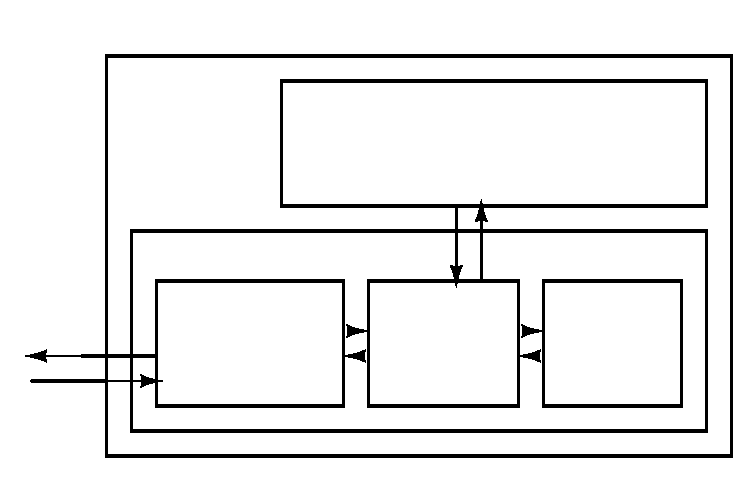
\includegraphics[scale=1]{../media/hbusdevice.ps}\\
   % translate x=616 y=512 scale 0.38
   \putbox{0.85in}{1.39in}{1.20}{Pilha HBUS}%
   \putbox{0.85in}{2.47in}{1.20}{}%
   \putbox{2.35in}{2.22in}{1.20}{Codigo específico}%
   \putbox{2.60in}{1.97in}{1.20}{do dispositivo}%
   \putbox{0.93in}{0.81in}{1.20}{\;\;Comunicação}%
   \putbox{2.51in}{0.81in}{1.20}{Objetos}%
   \putbox{0.68in}{2.81in}{1.20}{Dispositivo HBUS}%
   \putbox{3.68in}{0.89in}{1.20}{Micro}%
   \putbox{3.68in}{0.72in}{1.20}{código}%
   } % close 'parbox'
   } % close 'scalebox'
   \vspace{-\baselineskip} % this is not necessary, but looks better
\end{center}
